\documentclass[a4paper,10pt]{book}\usepackage{graphicx}
\usepackage{epstopdf}
\epstopdfsetup{update} % only regenerate pdf files when eps file is newer
\usepackage[utf8]{inputenc}
\usepackage{graphicx}
\usepackage{hyperref}
\usepackage{float}
\usepackage{tabularx}
\usepackage{pdfpages}

\restylefloat{table}
% Title Page
\title{Exam Report Communication Networks II}
\author{Daniel Plöger, Nina Piontek}

\begin{document}
\maketitle
\tableofcontents



\chapter{Network Description}
By Nina Piontek.\\

Because of a construction site near Channel 4 which might accidentally damage the cables 
used for internet connection,
a point-to-point radio link should be implemented to ensure network connection.
In the following, the new network configuration as depicted in \ref{fig:network} will be evaluated.
\begin{figure}[!ht]
  \begin{center}
    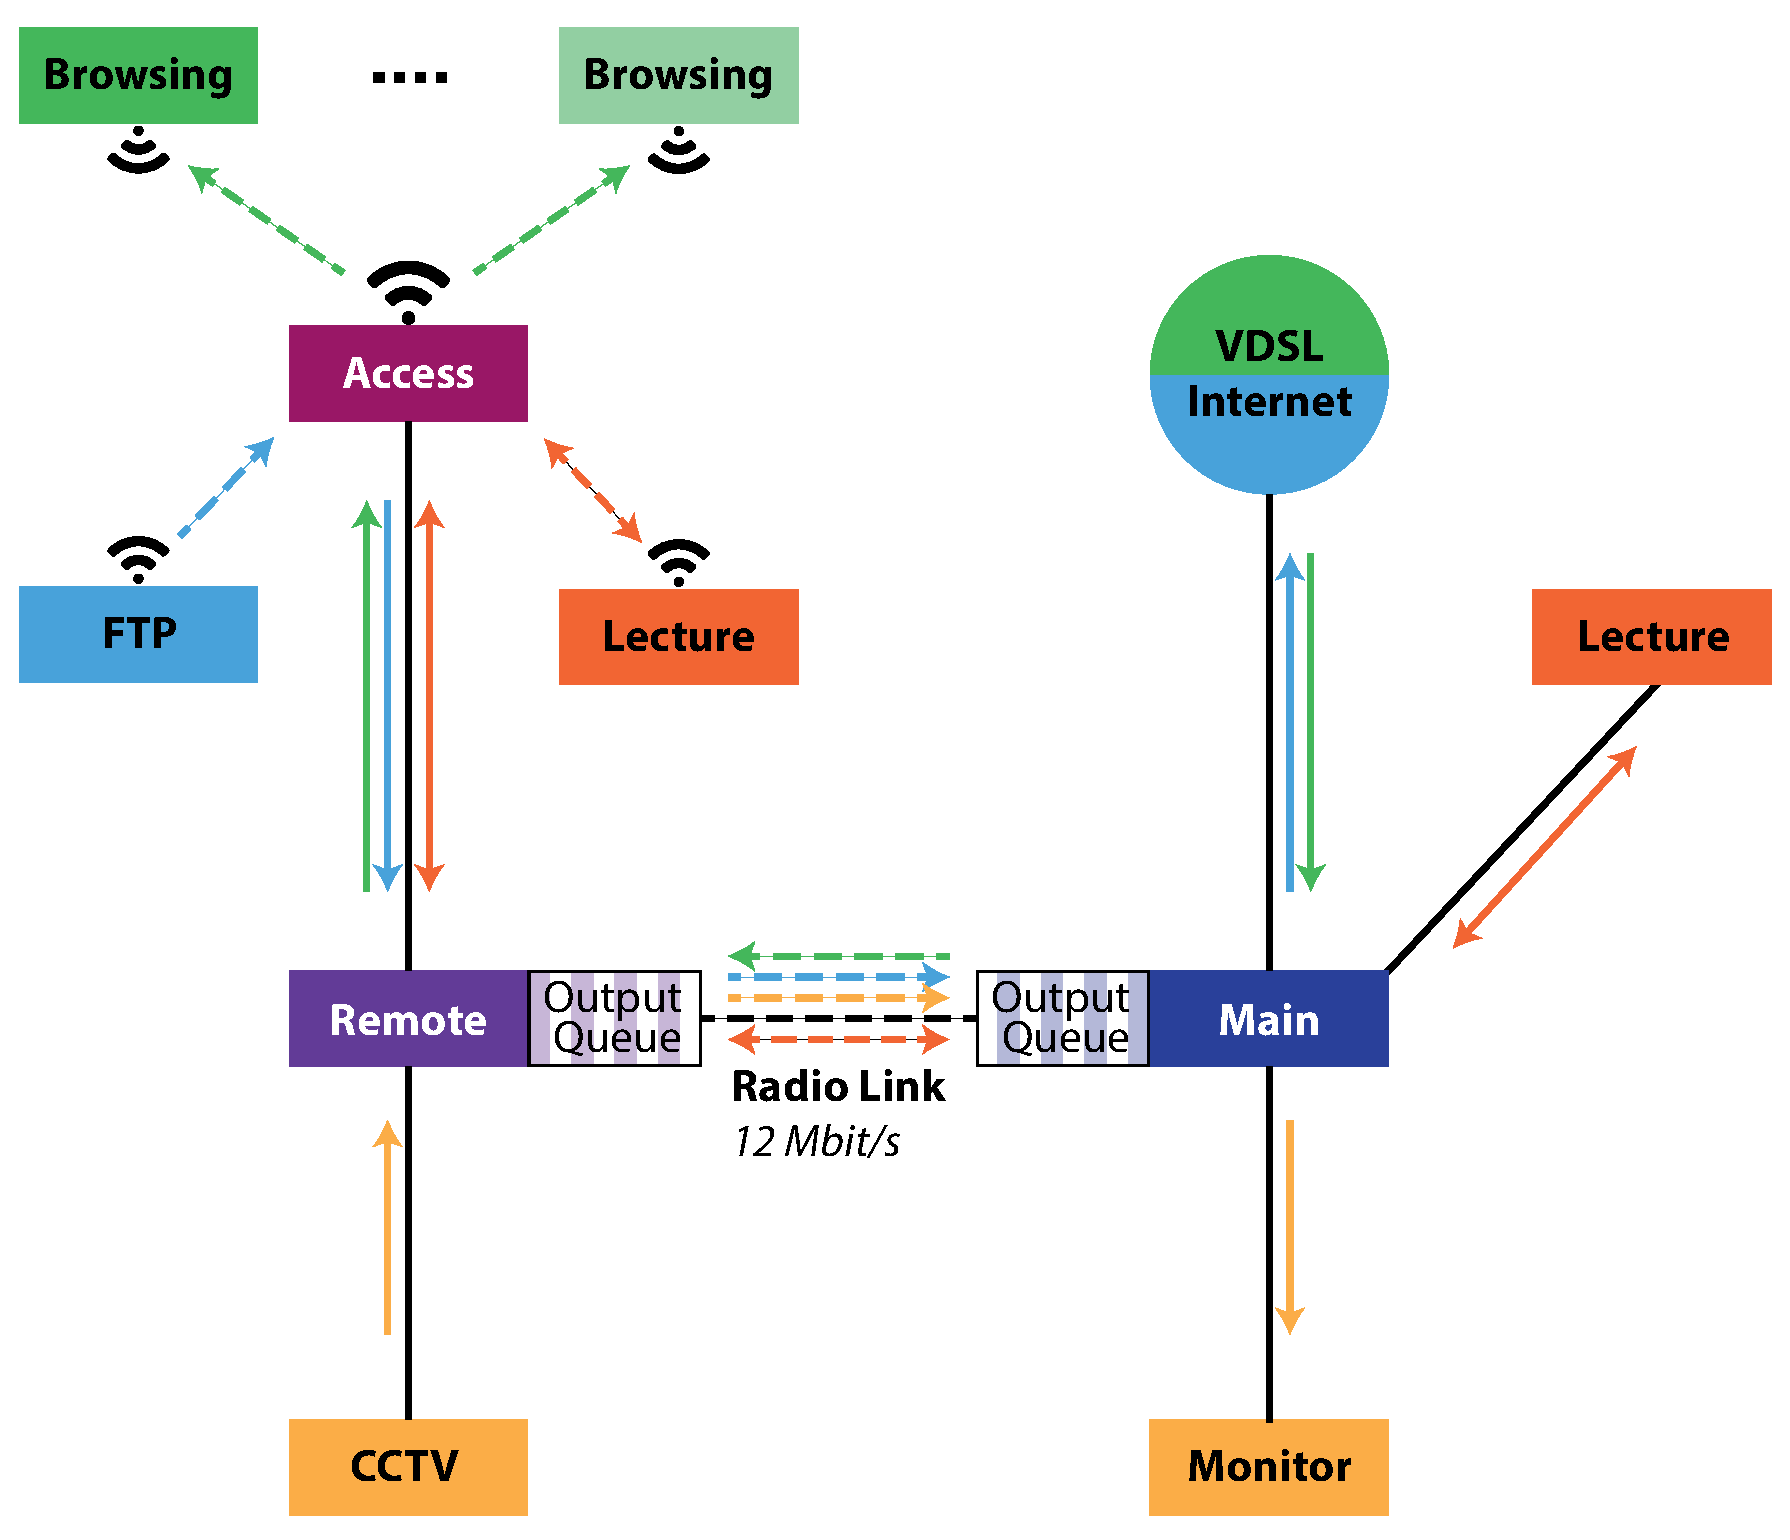
\includegraphics[width=0.9\textwidth]{graphics-03.eps}
    \caption{University Network with a remote site connected by the remote router (purple) and a main campus connected by the main router (navy blue)}
    \label{fig:network}
  \end{center}
\end{figure}

\section{General Description of the Network's Main Components}

The network core is a setup with 2 routers, main router and remote router, connected with a point-to-point link. 
Towards the main router the porters office's computer and the computer of the professor giving the remote lecture are connected.
The main router is the gateway for the shared internet connection of the university.

Towards the remote router the access point for WLAN and the security camera are connected.
The access point provides Wireless Lan for students at Channel 4. The computer for the video lecture at Channel 4 
is connected via WLAN as well.

\section{Network Services and Requirements}

In this set up the Network performance regarding the video lecture is evaluated with the following services in
use:\\
\begin{enumerate}
 \item WLAN for webbrowsing
 \item FTP service for uploading a file to a server in the internet (used by one student) 
 \item Video lecture streamed in both directions from the main Campus to channel 4
 \item Security camera streaming from Channel 4 to the porter's office  at the main campus
\end{enumerate}

The network should provide a certain Quality of Service for the video lecture and the security camera.
The criteria are:\\
\begin{enumerate}
 \item The video data should not take more than 100ms to be delivered to the destination in both directions.
 \item There should only be a loss of data of at most $5\%$.
\end{enumerate}

\chapter{Network Modeling}
\section{General Assumptions on the Model}
By Nina Piontek.\\

Since the overall goal is to evaluate the network performance regarding the QoS during the video lecture, we will assume an assessment period
of around 90 minutes. The WLAN at Channel 4 will in general be used by the students, which surf the web during the video lecture and the student 
who uploads a file. Optional the camera will be switched on or switched off to evaluate the networks behavior with and without the additional
traffic load.

\subsection{HTTP Traffic}
\label{chapter_http_traffic}
By Daniel Plöger.\\

In order to model the student web browsing behavior in 
a meaningful way, captured browsing statistics have been provided by the computer center in a trace file. 
This chapter shortly explains the statistical behavior behind the given HTTP 
requests and responses. The response sample traces (download statistics) are widely 
distributed in the range of less than 500 Bytes up to more than 4 Mbyte 
(see figure \ref{fig:trace} top).
\begin{figure}[!ht]
  \begin{center}
    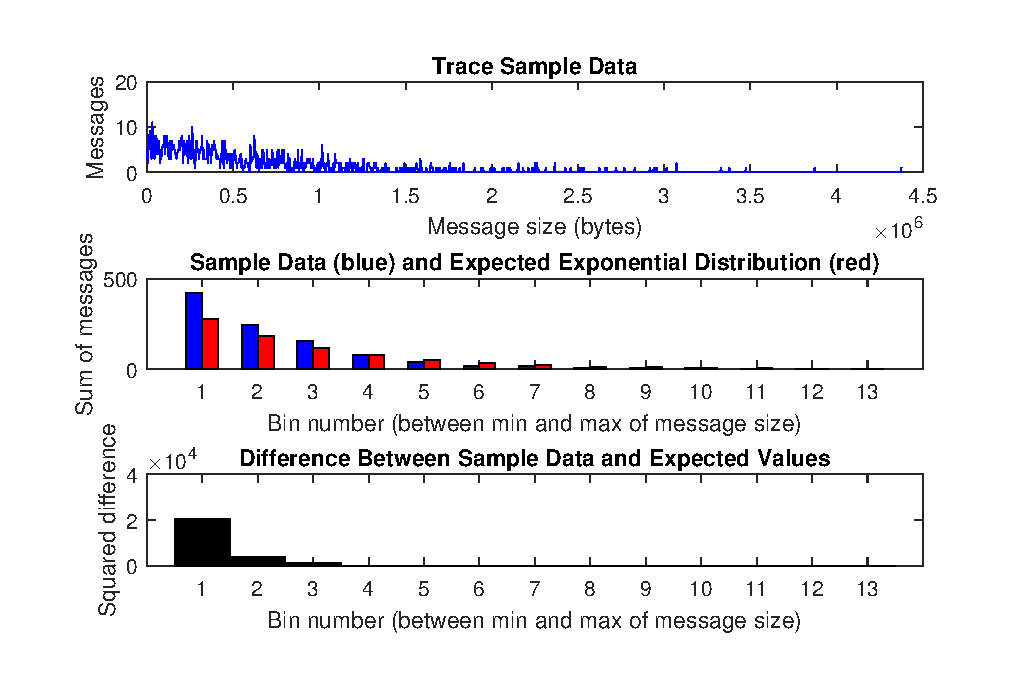
\includegraphics[width=0.9\textwidth]{trace_distribution.eps}
    \caption{HTTP Traffic Analysis}
    \label{fig:trace}
    \end{center}
\end{figure}

Distribution fitting analysis shows that the statistical behavior if
 partitioned in a smaller number of bins roughly behaves like a negative 
exponential distribution with a mean value of 0.789 Mbyte (see figure \ref{fig:trace} center) \cite{goodness_of_fit}. 
The phrase "roughly" means that while the statistical goodness of fit tests accepts
 this distribution, the actual data has an overweight of small messages compared to
 the expected values (see figure \ref{fig:trace} bottom). An exponential distribution with the
 mean of 0.789 Mbyte is used in this report for simulation nonetheless. 
This is a conservative approach and guarantees an upper bound in the distribution:
 if the actual browsing behavior uses smaller HTTP responses with a slightly higher
 probability, the QoS assumptions from the following chapters are going to be met 
in practice as well.
\section{Network Behavior  Expectations without CCTV camera}
By Nina Piontek.\\

\begin{table}[ht]
\centerline{
\begin{tabular}{|l|l|l|l|l|}
\cline{1-4}
 \textbf{Link} & \textbf{Data Rate}  & \textbf{Downlink}  & \textbf{Uplink}  \\ \cline{1-4}
 WLAN & 54Mbit/s  & HTTP, Video Lecture & FTP,Video Lecture \\ \cline{1-4}
 Access Point $\leftrightarrow$ Remote Router & 100Mbit/s  &HTTP, Video Lecture& FTP  \\ \cline{1-4}
 Camera $\leftrightarrow$ Remote Router & 100Mbit/s  & - & Camera\\ \cline{1-4}
 Remote Router$\leftrightarrow$Main Router&12 Mbit/s&HTTP,Video Lecture& FTP, \\ 
 & & & Video Lecture, Camera \\ \cline{1-4}
 Main Router$\leftrightarrow $ Porters Office &Ideal Connection &Camera& - \\ \cline{1-4}
 Main Router$\leftrightarrow $ Professor & -  &Video Lecture&Video Lecture \\ \cline{1-4}
 Main Router$\leftrightarrow $ Internet &100Mbit/s &HTTP& FTP \\ \cline{1-4}
\end{tabular}}
\end{table}

The performance of the uplink and the downlink is evaluated independently because the default configuration for the links is full-duplex. When the camera is switched off, the uplink to the main campus is shared between the FTP upload and the video lecture (video conference). The video conference is sending with a constant data rate of 280 kbit/s, the remaining 11,72 Mbit/s can be used by the FTP upload. 

\begin{figure}[!ht]
  \begin{center}
    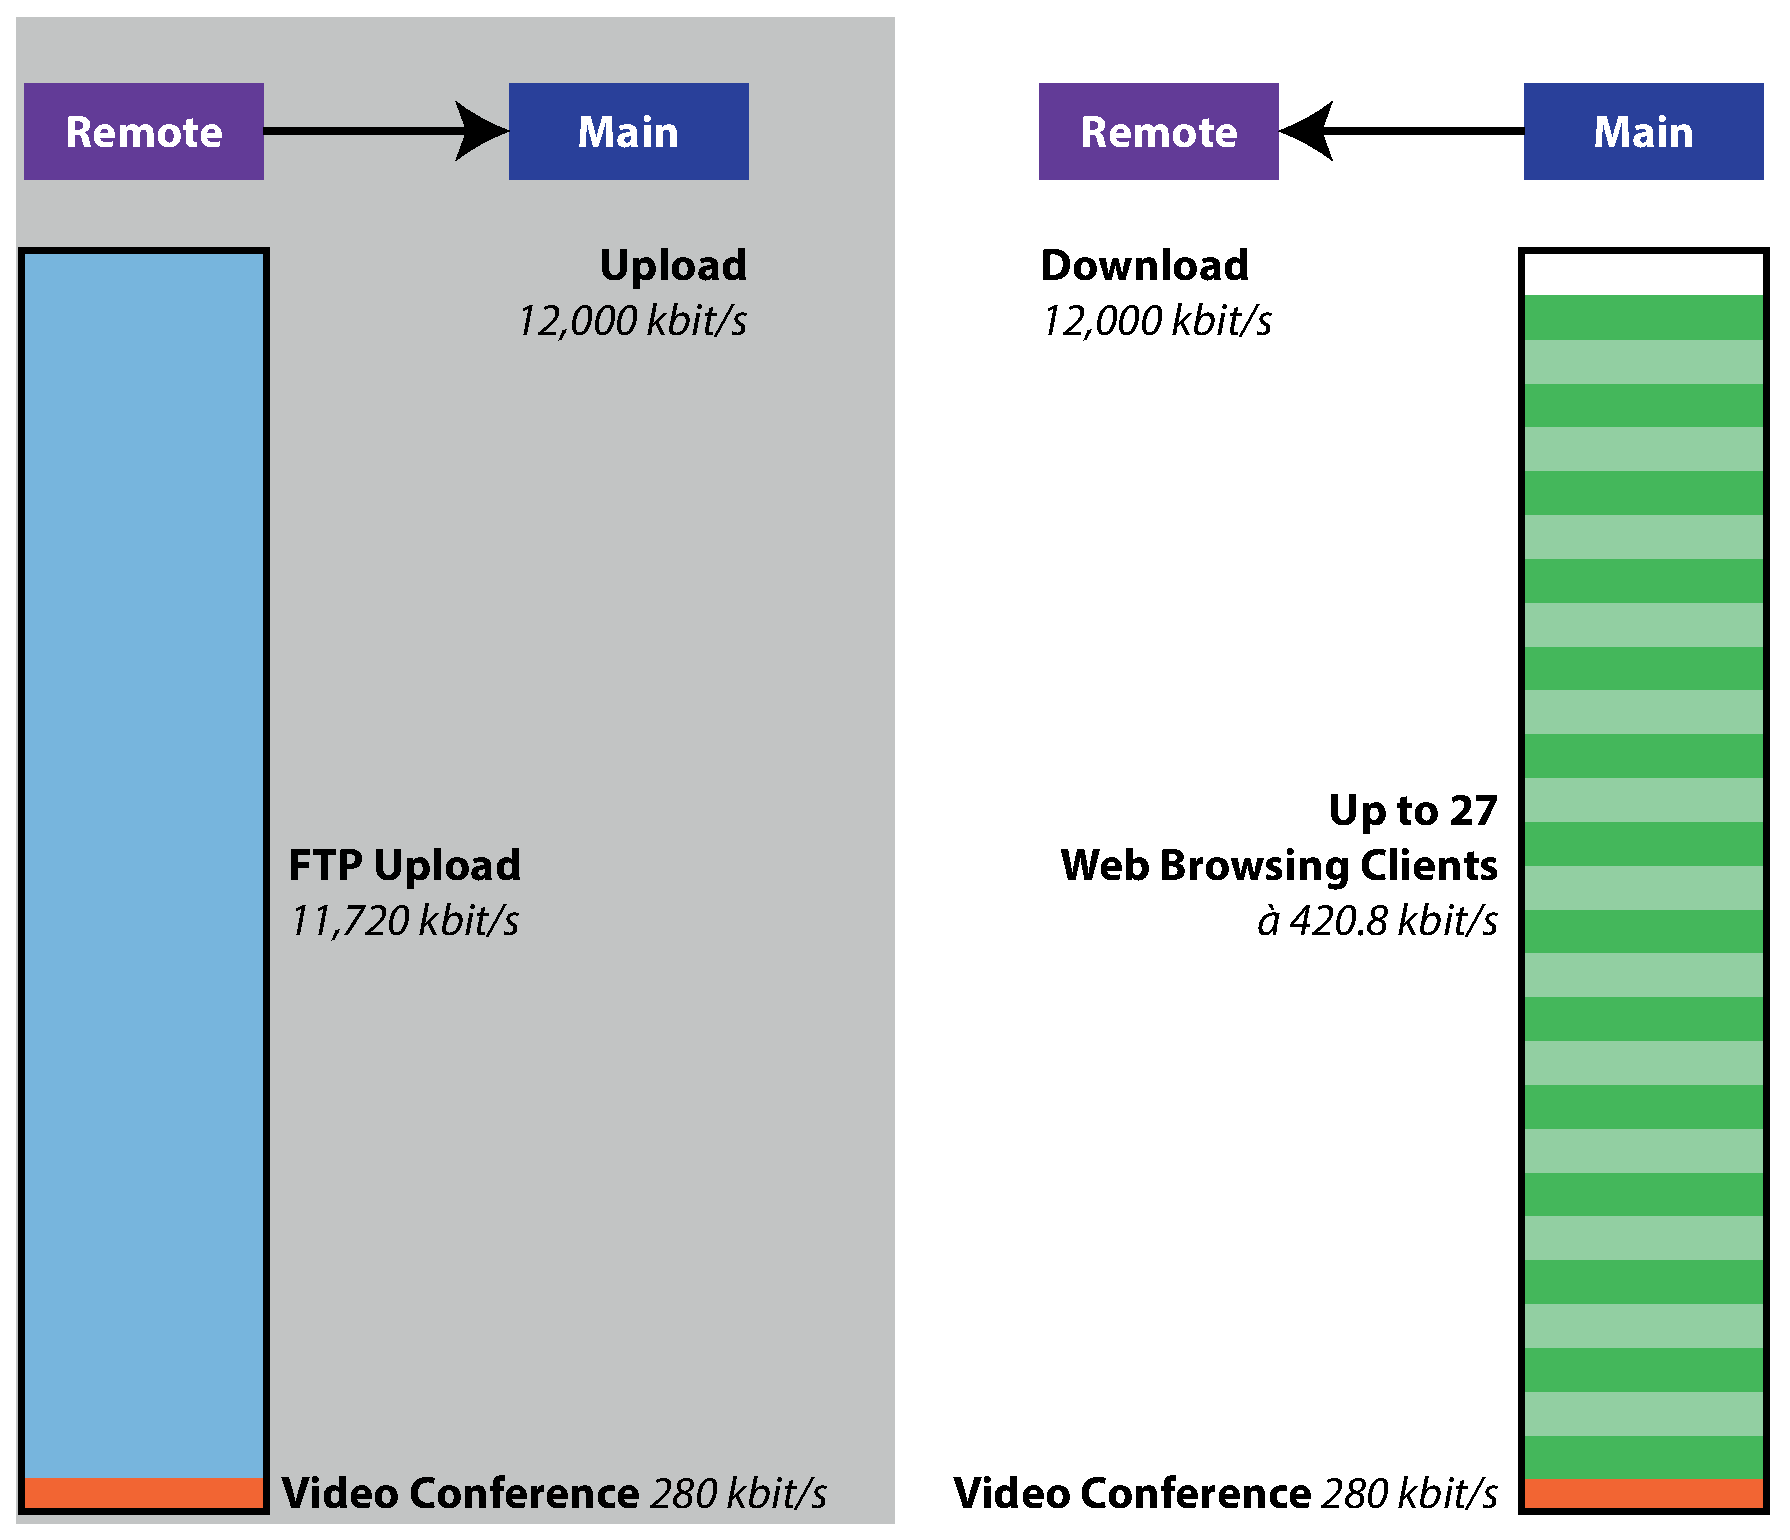
\includegraphics[width=0.9\textwidth]{graphics-02.eps}
    \caption{Utilization of the Radio Link without the Security Camera}
    \label{fig:rLink}
    \end{center}
\end{figure}

On the downlink the data rate of 12 Mbit/s is shared between the students browsing the web (HTTP service) and the video lecture (video conference).
The Downlink is utilized by the Video Lecture by 280kbit/s , the remaining 11,72 Mbit/s can be theoretically used by the HTTP service. With 
\begin{equation}
 \frac{0.789 MiB}{15s}=\frac{441.24 kbit}{s}
\end{equation}
we can see, that, theoretically, up to 26 users can use the downlink for HTTP traffic. The value $0.789MiB$ is the value extracted from the trace file. It is the mean of the packetlength downloaded by the students when surfing the web. For details see~\ref{chapter_http_traffic}.

\section{Network Behavior Expectations with CCTV Camera Turned On}
\label{chapter_expectations}
By Daniel Plöger.\\

The point-to-point radio link between remote and main router has a full duplex data rate of 12 Mbit/s and by this is the weakest single link within the proposed network. All other connection speeds are multiples of this data rate. Since all data has to pass this link, for this theoretical behavior analysis it is considered to be the network bottleneck.
\begin{figure}[!ht]
  \begin{center}
    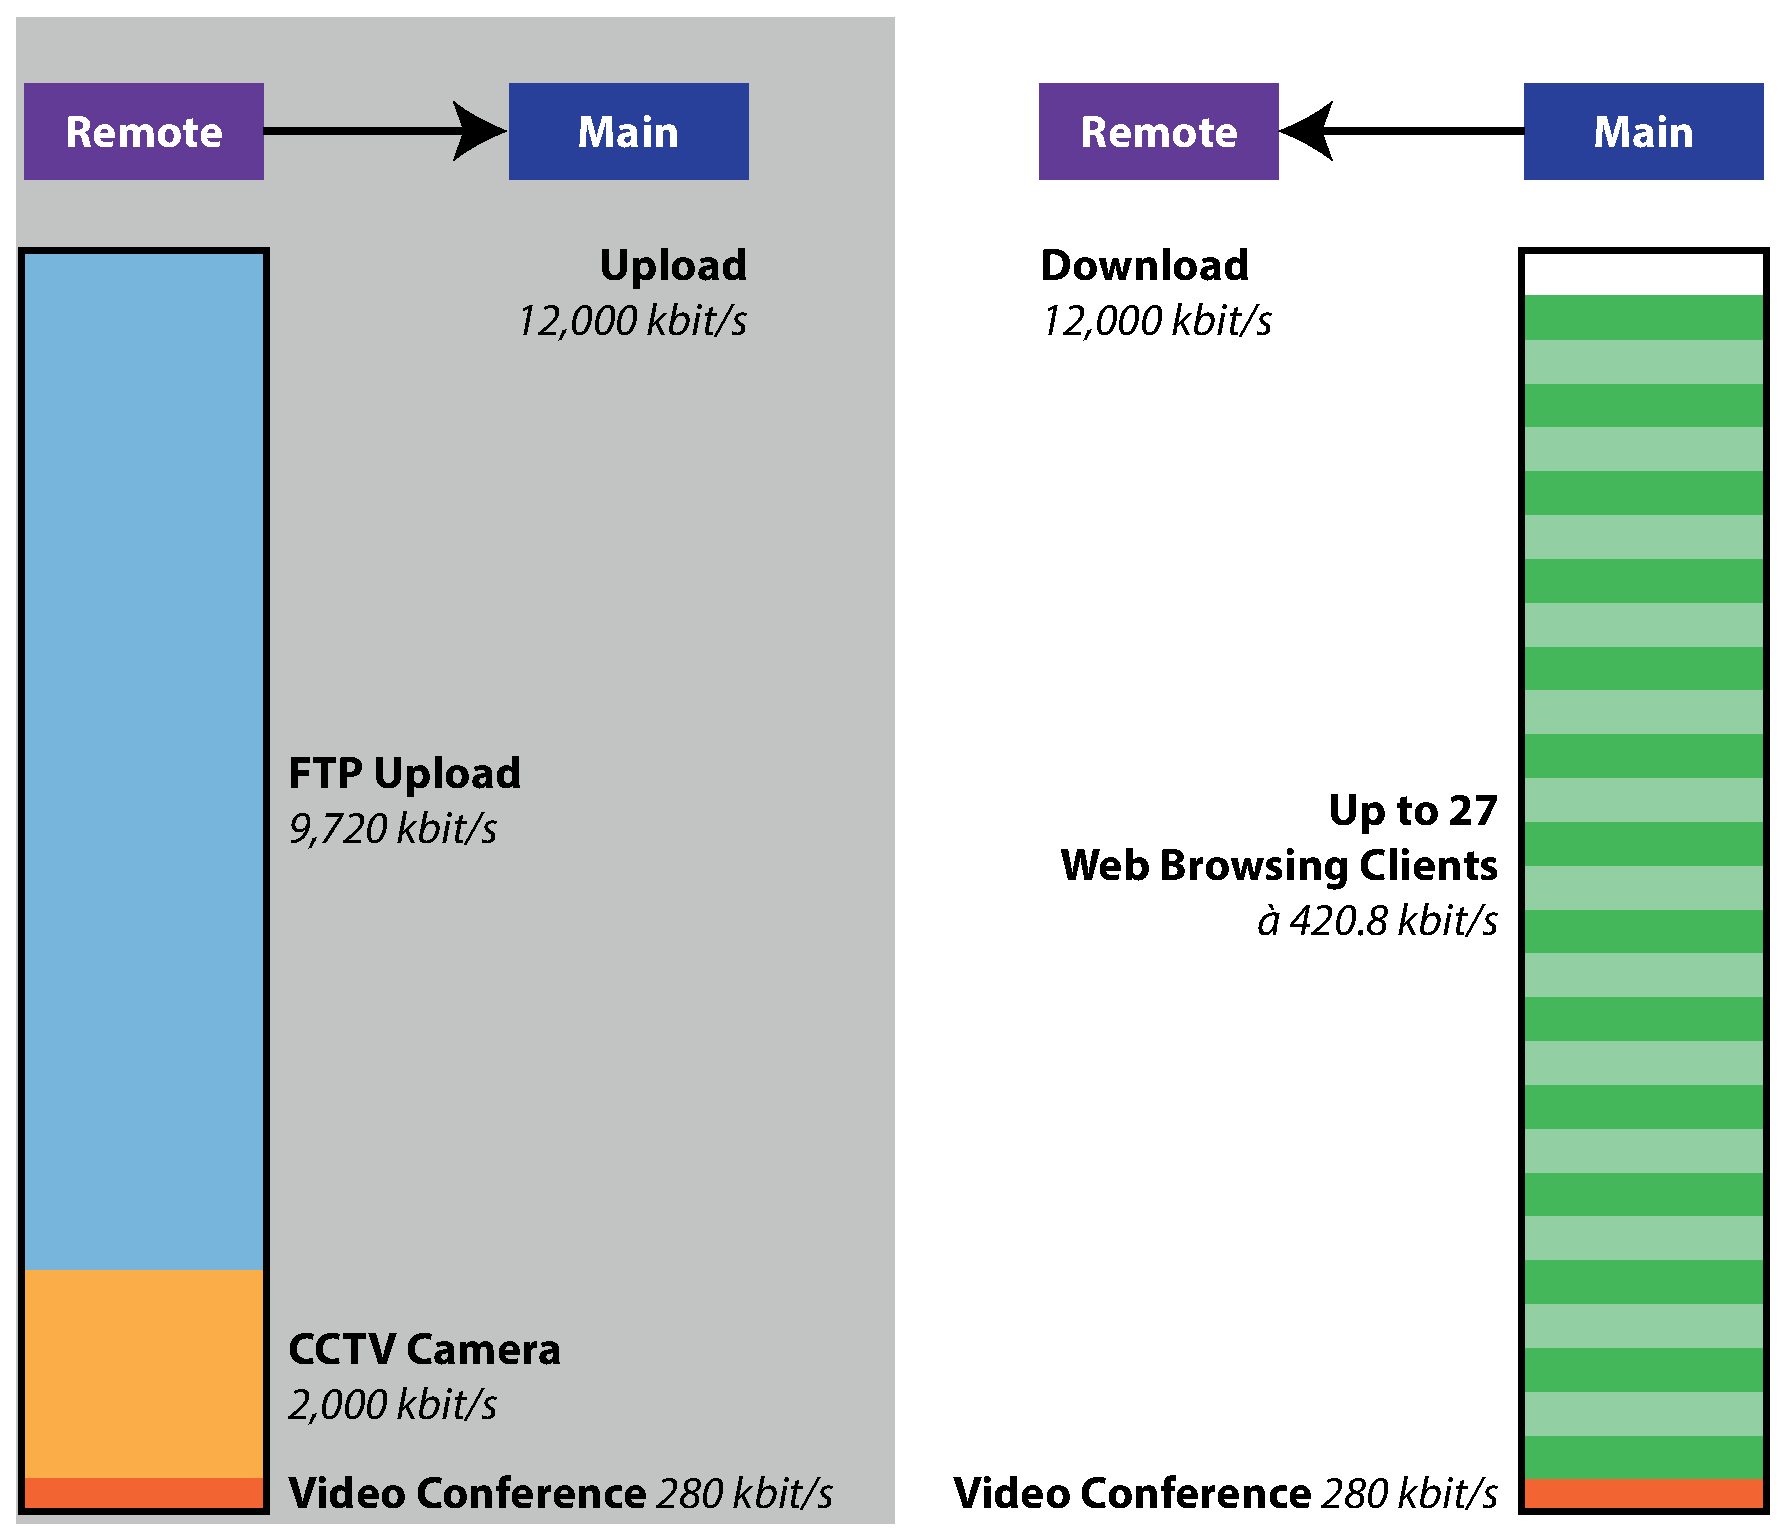
\includegraphics[width=0.9\textwidth]{graphics-01.eps}
    \caption{Max. possible utilization of upload (left) and download (right) of the radio link with the CCTV camera streaming.}
    \label{fig:radioLinkTheoryOn}
    \end{center}
\end{figure}

The network contains several applications which have their main impact either on the download connection from the main router to the remote router, or on the upload connection in the other direction. The respective opposite direction of an application may be neglected, since it mainly consists of very small messages for connection management or empty network packets. For this reason, theoretical down- and upload utilization is examined independently from each other in this chapter. 

The only exception is the video conference, which utilizes both, up- and download equally. The video stream consumes 280 kbit/s for transmission of 1388 Bytes of payload plus 12 Byte RTP protocol headers. It does this every 40 ms and in both directions.

\subsection{Upload Connection, Remote to Main Router}
Aside from the video conference which uses 280 kbit/s, two more applications make use of the upload direction. Firstly, the CCTV camera sends 10 kByte every 40 ms, which adds up to 2,000 kbit/s. The second application is the FTP upload. It tries to maximize network utilization and should therefore consume the biggest part of the remaining 9,720 kbit/s of the total 12,000 kbit/s data rate (see figure \ref{fig:radioLinkTheoryOn} left).

\subsection{Download Connection, Main to Remote Router}
Other than the video conference, the only application which makes use of the download direction is the web browsing. As stated before, web browsing is modeled as the download of files with an exponentially distributed size with a mean of 0.789 Mbyte (see chapter \ref{chapter_http_traffic}). The client's assumption states that a web browsing user waits a certain time before he downloads the next file. The waiting time is assumed to be exponentially distributed with a mean of 15 seconds. This leads to an expected average data rate of 420.8 kbit/s per user. Therefore, if all users download in a well-distributed way, up to 27 users are able to browse simultaneously via the network connection (see figure \ref{fig:radioLinkTheoryOn} right).

\subsection{Conclusion}
For a fully-functional network that guarantees both the CCTV camera and the video lecture conference to satisfy all quality of service requirements, the proposed network is not able to allow for many additional applications or users. In theory, a classroom in the given size could host up to 800 tightly seated students for lecture \cite{sitzkultur}. The expected behavior suggests that in theory up to 27 of them are able to browse the web at the same time without restricting the video streams. 

In practice however the network is expected to permit even less simultaneous users. This is due to the nature of HTTP requests and responses: the requested data is not perfectly distributed over time. Instead, high peaks of transmitted data occur at certain points in time, alternated with moments of complete silence. The video streams on the other hand are expected to transmit reliably at any point in time.

Meanwhile, the FTP upload and the CCTV camera stream is expected to be mostly independent of the number of web clients. The main transmission direction of these applications is upwards from the remote site to the main campus, opposite to the web browsing downloads. With higher numbers of web clients, the uploads are expected to slow down very little only due to the rising number of session handling messages from the underlying protocols.

\chapter{Evaluation Without Camera}
By Nina Piontek.\\

\subsection{Simulation Results}
\section{Video Lecture}
The overall goal is to ensure a good Quality of Service for the video lecture in both directions.
A good Quality of Service is achieved, if there are only up 5 $\%$ loss of data
on the way from the professor's laptop to the students watching the lecture in Channel 4. Also the average delay of data travelling from the professor to the students has to be smaller than 100ms.
Data loss (named packet loss in ~\ref{fig:losslecdown}) occurs, when the traffic load on the network is too high, and the network nodes cannot process all packets.
The data is then dropped. Data is delayed for example by queuing at routers.
In figure  ~\ref{fig:losslecdown} the packet loss rate depending on the number of
webusers is depicted. Packet loss is calculated with
\begin{equation}
 \frac{\textnormal{total number bits sent}}{\textnormal{total number of packets received}} + \textnormal{number of packets arrived at time} > 100ms
\end{equation}
The packet loss should not exceed 5$\%$ during the simulation.
With increasing number of users, the packet loss increses, because the 
workload on the network nodes like routers is too high.
The simulation results indicate, that the maximum number of clients surfing the 
web without impairing the video lecture is about 7 users.
The blue lines indicate the confidence intervals. Confidence intervals give the area in which 
the true mean of the probability distribution that underlies the gathered data will lie with a probability of 90$\%$.
The mean we are estimating is the average packet loss rate. The estimated mean taken from the simulation results is depicted in the figure with a blue star.
The estimated mean lies within the calculated confidence intervals for each number of users. This indicates that the estimated mean is a good estimate of the true mean.
It is safe to assume that only 6 users can use the web, while the video lecture is running.
The confidence interval for 6 users does not cross the 5$\%$ acceptable packet loss 
rate indicated by the red line. So the Quality of Service is guaranteed with a probability of 90$\%$, because the actual mean of the
underlying distribution will have its mean in the depicted interval with a probabiity of 90$\%$.
data is caused by collisions during transmission from Access Point to Wlan clients.

Investigating the source of the packet drops, figure ~\ref{fig:mainRdrops} shows the packet drops at the main router, which increase with the number of 
web users. With increasing webusers more data are lost at the main router and the Quality of Service for the video lecture decreases. Further investigation of the loss rate at the access point showed no indication that 
the loss of data is caused by collisions during transmission from access point to WLAN clients.

\begin{figure}[!ht]
  \begin{center}
    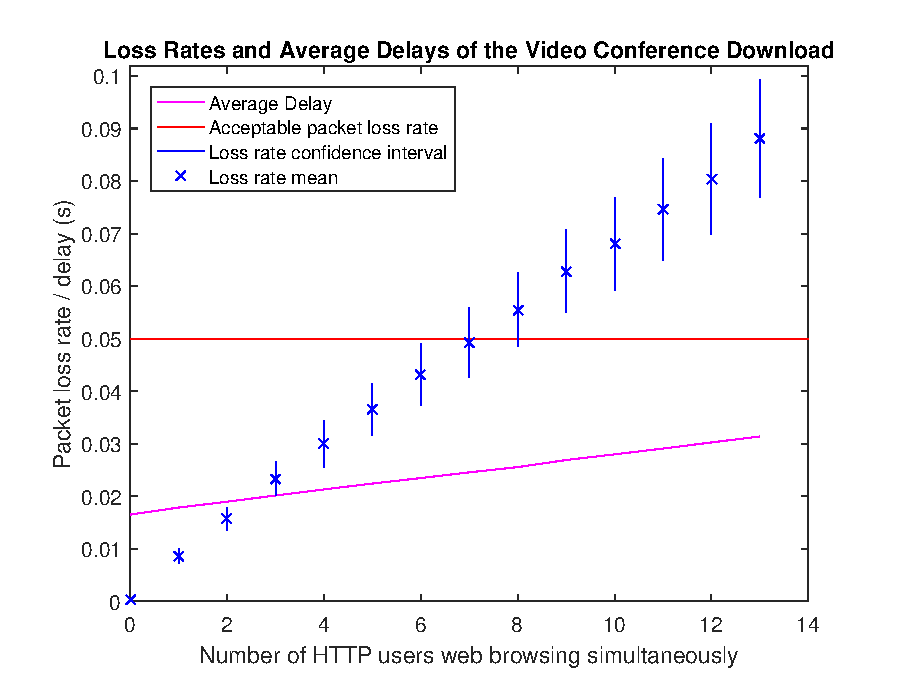
\includegraphics[width=0.9\textwidth]{off_loss_conf_download.eps} 
    \caption{Loss Downlink}
    \label{fig:losslecdown} 
  \end{center}
\end{figure}
The bootleneck of that configuration without the security camera constantly streaming to the main campus 
is the radio link.
\begin{figure}[!ht]
  \begin{center}
  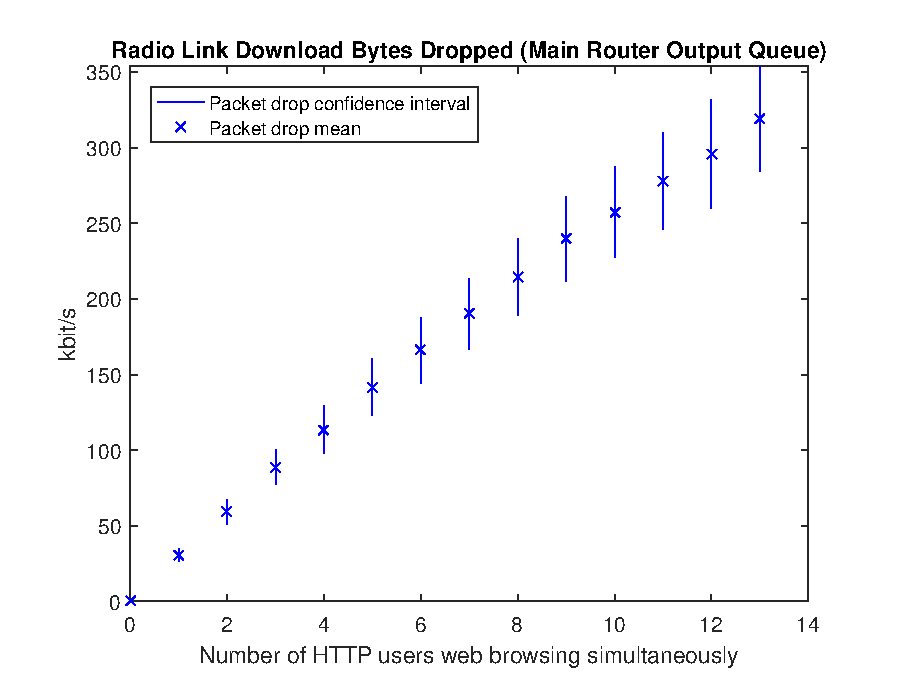
\includegraphics[width=0.9\textwidth]{off_main_router_drops.eps}
    \caption{Drops main router (downlink)}
  \label{fig:mainRdrops}
  \end{center}
\end{figure}

In the uplink, there is no loss of data at the remote routers queue on the radio link (see~\ref{fig:remoteRdrops}).
This means no impact on the Quality of Service for the video lecture (see~\ref{sec:ftp}).
\begin{figure}[!ht]
  \begin{center}
  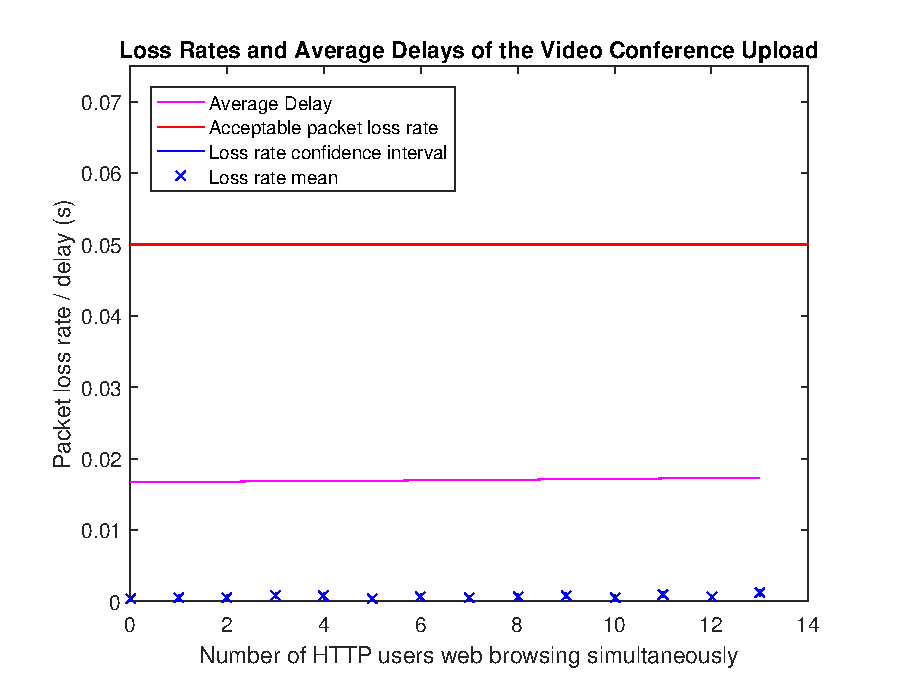
\includegraphics[width=0.9\textwidth]{off_loss_conf_upload.eps}
    \caption{Loss uplink}
     \label{fig:losslecup}
     \end{center}
\end{figure}

\begin{figure}[!ht]
  \begin{center}
    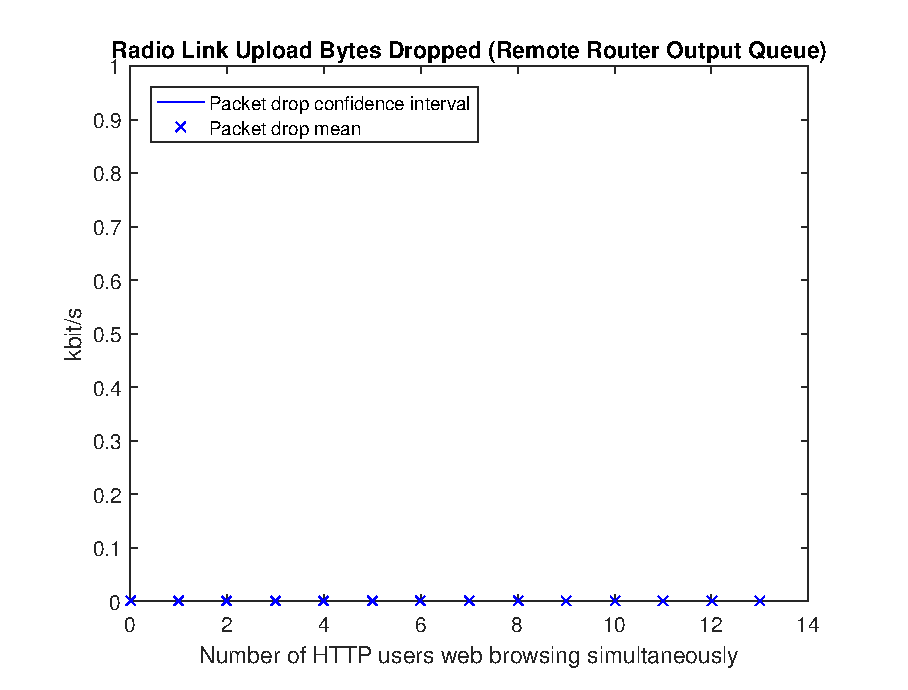
\includegraphics[width=0.9\textwidth]{on_remote_router_drops.eps}
    \caption{Drops remote router (Uplink)}
     \label{fig:remoteRdrops}
     \end{center}
\end{figure}

\section{Problems with FTP}
\label{sec:ftp}
The networks behaviour on the uplink is very unusual. Since the FTP client uploading a file is using TCP it therefore adjusts its upload speed if the network can provide a higher datarate.
As we can see in ~\ref{fig:ftpUpR}, the FTP Client starts with an average upload rate of around 1250 kbit/s , despite the fact, that it could theoretically transmit with a datarate of up  11,7 Mbit/s.
The Video Conference is using UDP and sending with constant datarate of 280 kbit/s without adjusting its upload rate. This means, that the FTP client really has 11,7 Mbit/s for upload. The Problem might be our implementation of the FTP upload. 

\begin{figure}[!ht]
  \begin{center}
    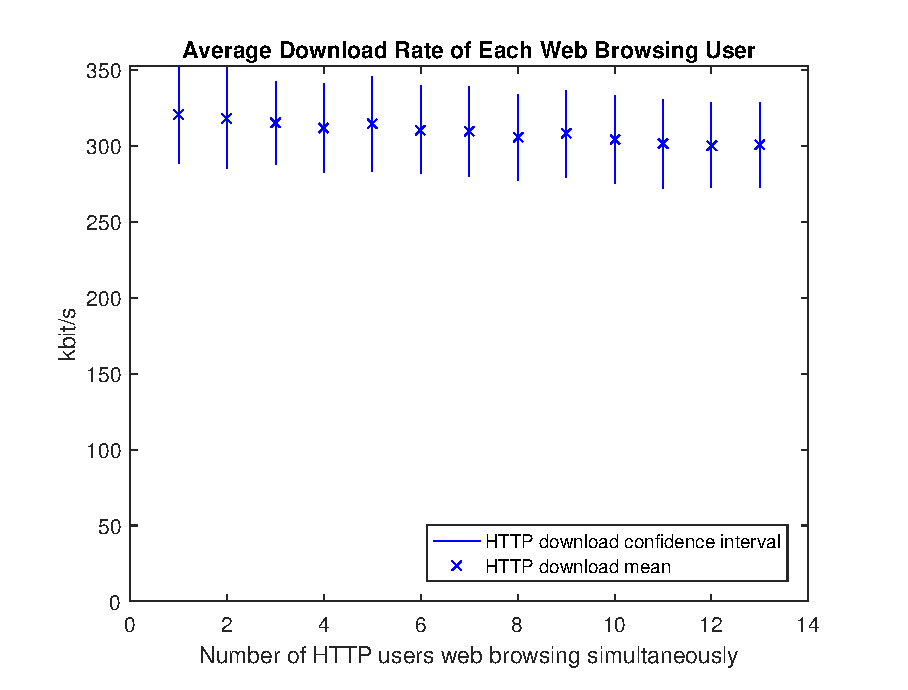
\includegraphics[width=0.9\textwidth]{off_http_download.eps}
    \caption{Average download rate depending on number of Users surfing the web}
    \label{fig:httpDR}
  \end{center}
\end{figure}

\begin{figure}[!ht]
  \begin{center}
    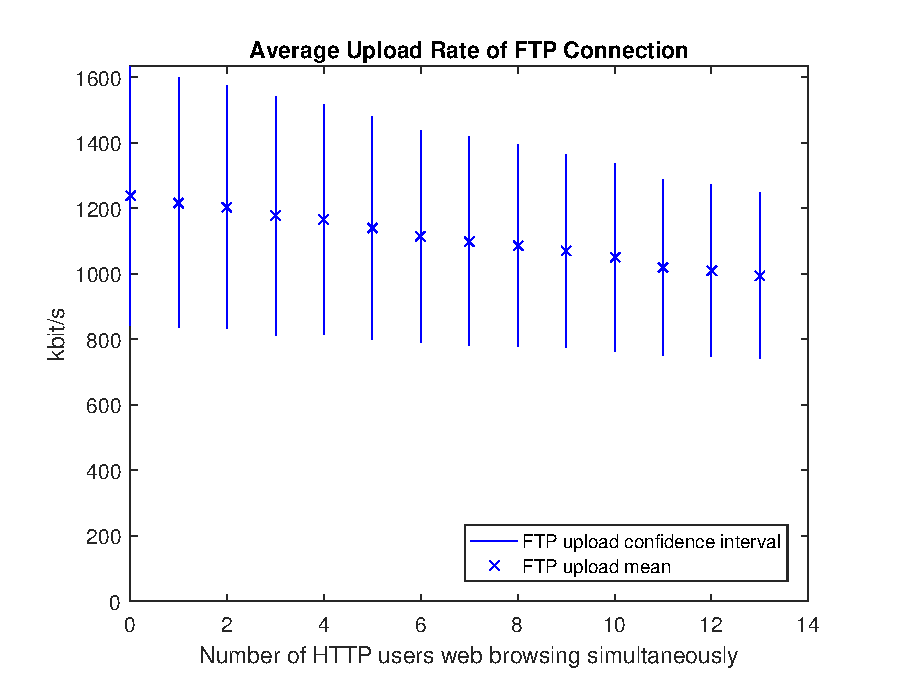
\includegraphics[width=0.9\textwidth]{off_ftp_upload.eps}
    \caption{Average upload rate for the FTP upload depending on the number of users}
    \label{fig:ftpUpR}
  \end{center}
\end{figure}

\section{Webbrowsing}
As we can see in \ref{fig:httpDR} with increasing number of students using the WLAN for webbrowsing, the average download rate decreases only slightly over time. Webbrowsing is still possible, but with decreased download speed.
To provide a higher download rate the data rate of the radio link has to be increased. 

\chapter{Evaluation With Camera Turned On}
By Daniel Plöger.\\

In order to assess the proposed network, the behavior was simulated and will be evaluated in this chapter. The evaluation is divided into the sections \textit{loss rates and delays analysis}, \textit{HTTP data rates}, \textit{FTP data rate}, and \textit{main bottlenecks}. In each section, the results are examined with regards to the number of HTTP users that are web browsing simultaneously and compared to the expected behavior from chapter \ref{chapter_expectations}. This is because the main aim of the evaluation is to show how the quality of service of the video streams changes with the number of HTTP users. 

The total packet drop rate plus the rate of packets exceeding 100 ms in delay must not be more than 5\% for the quality of service to be satisfied. This combined drop-and-delay-rate will be called \textit{packet loss rate} in this chapter. The network is simulated with up to 13 HTTP users instead of up to 27 as suggested in the theoretical analysis. It will be seen that the network is already working to capacity with less users. In addition to the mean loss and data rates, the evaluating figures indicate intervals inside which all actual values stay with 90\% confidence.

\section{Loss Rates and Delays Analysis}

The conference stream of the video lecture is analyzed in both directions. In the upload from the remote classroom to the professor's laptop, the video quality-of-service is not becoming worse with more number of users (see figure \ref{fig:onLossConfUpload}). The loss rate is  negligible the whole time. This was predicted in the expected performance, since the direction of the video upstream is opposite to the HTTP download. The average delay also stays constant below 20 ms, which is much less than the maximum acceptable 100 ms.

\begin{figure}[!ht]
  \begin{center}
    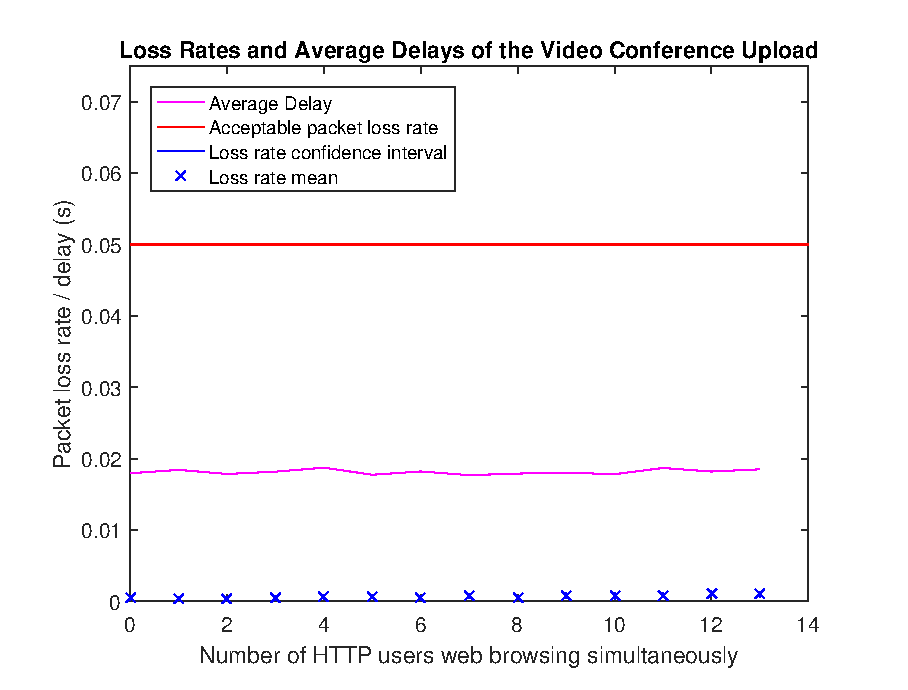
\includegraphics[width=0.9\textwidth]{on_loss_conf_upload.eps}
    \caption{Video conference upstream loss rates and delays depending on the number of HTTP users}
    \label{fig:onLossConfUpload}
  \end{center}
\end{figure}

\begin{figure}[!ht]
  \begin{center}
    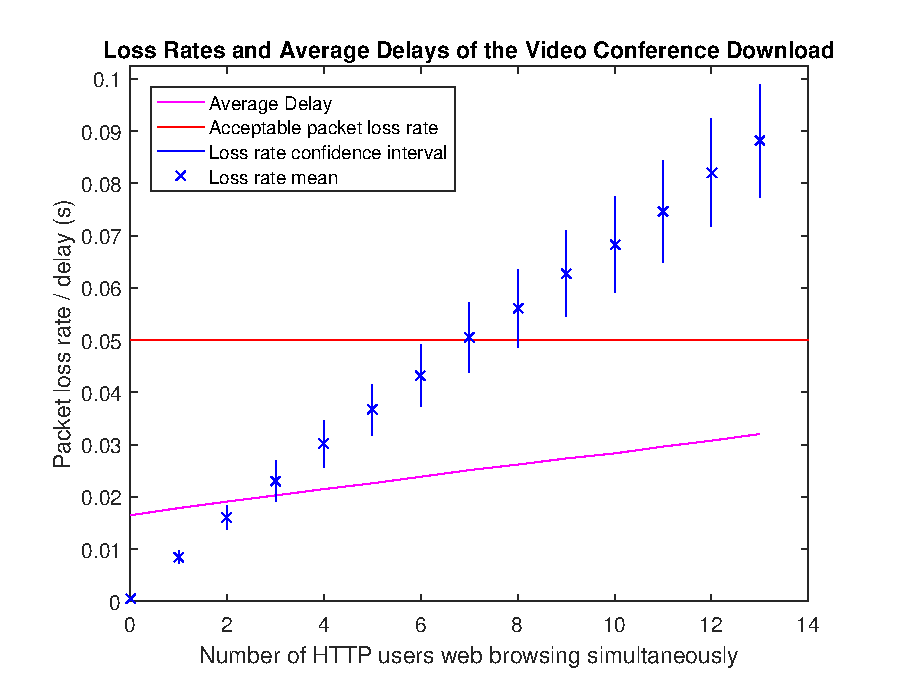
\includegraphics[width=0.9\textwidth]{on_loss_conf_download.eps}
    \caption{Video conference downstream loss rates and delays depending on the number of HTTP users}
    \label{fig:onLossConfDownload}
  \end{center}
\end{figure}

The download gives a different picture: with an increasing amount of users, the service quality approximately decreases linearly (see figure \ref{fig:onLossConfDownload}). While there is no video packet loss without any user, it can be used safely with up to six users, only. For a higher number the quality of service hits an unacceptable level. The average delay increases as well, but always stays on a safe level. This is a misleading however, as the delay variance increases a lot over time. For seven users, for example, the delay rate exceeding 100 ms is already above 4\%.

\begin{figure}[!ht]
  \begin{center}
    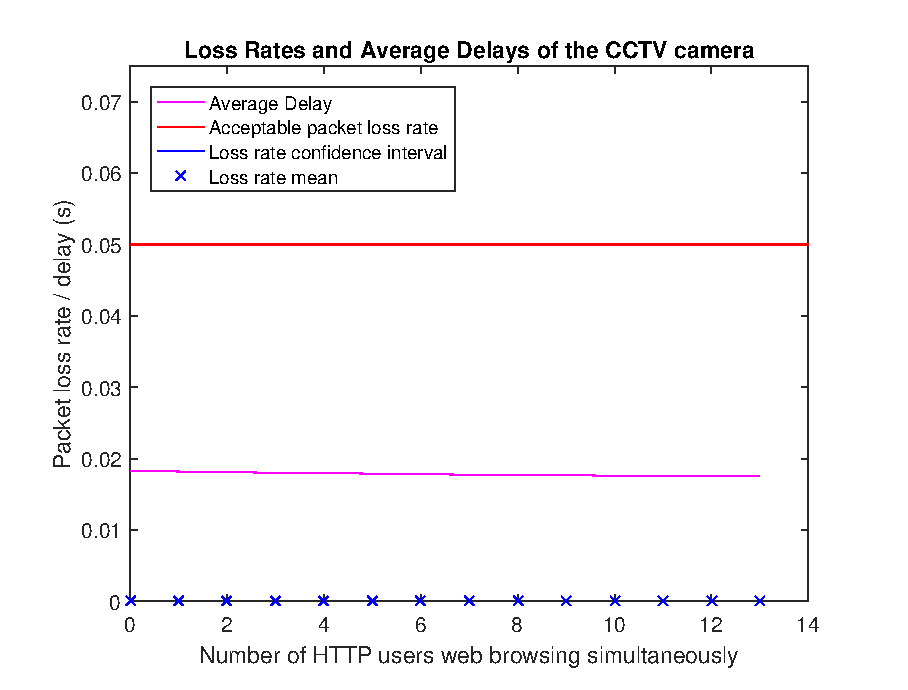
\includegraphics[width=0.9\textwidth]{on_loss_cctv.eps}
    \caption{CCTV video stream loss rates and delays depending on the number of HTTP users}
    \label{fig:onLossCctv}
    \end{center}
\end{figure}

Just like the video conference upstream, the CCTV camera stream is independent of the number of users (see figure \ref{fig:onLossCctv}). The loss rate is negligible for all number of users and the average delay stays close to the theoretical minimum of 10 ms.

\section{HTTP Data Rates}
\begin{figure}[!ht]
  \begin{center}
    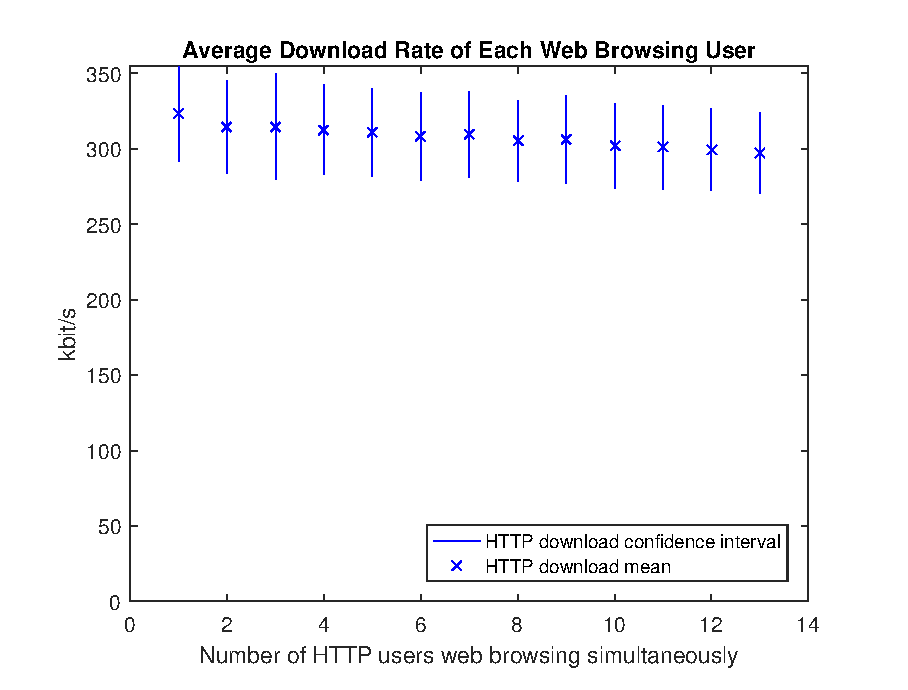
\includegraphics[width=0.9\textwidth]{on_http_download.eps}
    \caption{Average download rate per HTTP user depending on the total number of HTTP users}
    \label{fig:onHttpDownload}
    \end{center}
\end{figure}

The average download rate per web browsing user almost stays constant when the number of users increases (see figure \ref{fig:onHttpDownload}). On average, is stays between 350 and 275 kbit/s, which is more than two third of the expected theoretical download rate from chapter \ref{chapter_expectations}. This result indicates that the users have a comfortable web browsing experience for this number of clients. 

Only for overlapping peaks of downloads, the download speed will have to be shared between users and thus decreases notably. This leads to a minor drop on the time average between one and 13 users. While higher number of users were not simulated, the average download rate is expected to drop faster from around 27 HTTP users upwards. This is because with that number of users, the radio link bandwidth is filled to capacity not in peaks only but also on average.

\section{FTP Data Rate}
\begin{figure}[!ht]
  \begin{center}
    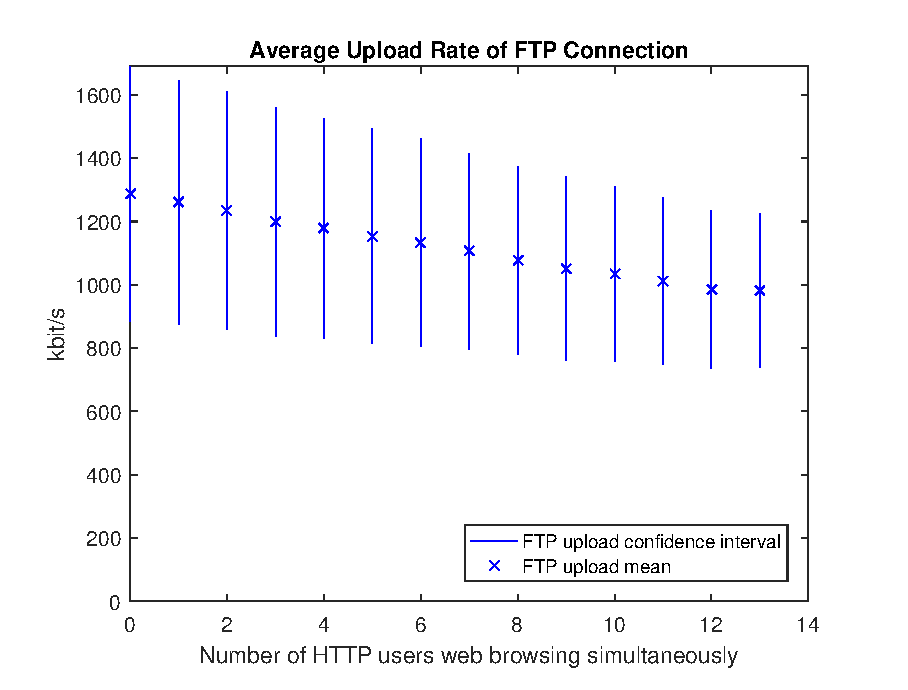
\includegraphics[width=0.9\textwidth]{on_ftp_upload.eps}
    \caption{Average upload rate of the FTP connection depending on the number of HTTP users}
    \label{fig:onFtpUpload}
    \end{center}
\end{figure}

FTP upload changes only little with the number of HTTP users increasing (see figure \ref{fig:onFtpUpload}). Its mean value decreases from 1300 kbit/s without any web surfing down to 1000 kbit/s with 13 users. Just as expected, that the influence is so small can be explained by the direction within the network, which is opposite between web browsing data download and FTP upload. Only protocol handshakes and control data of the FTP connection may get stuck in queues together with the HTTP data and thus slows down the FTP upload.

The general speed of the FTP connection stays far below the expected data rate however. More about this topic in chapter \ref{chapter_conclusion} (conclusion).

\section{Main Bottlenecks and Conclusion}

The initially assumed bottleneck at the radio link connection proves true: the main router output queue buffers the packets which are waiting to be transmitted via the radio link. With six HTTP users active, around 175 kbit worth of packets are dropped each second (see figure \ref{fig:onMainRouterDrops}). The average throughput at this connection is 2,400 kbit/s with six users. This means that 7.3\% of all transmitted Bytes are lost at the main router only. The second worst packet drop rate belongs to the WLAN access point connections, which have average packet loss rates of around .6\%, only a fraction of the main router packet drops.

\begin{figure}[!ht]
  \begin{center}
    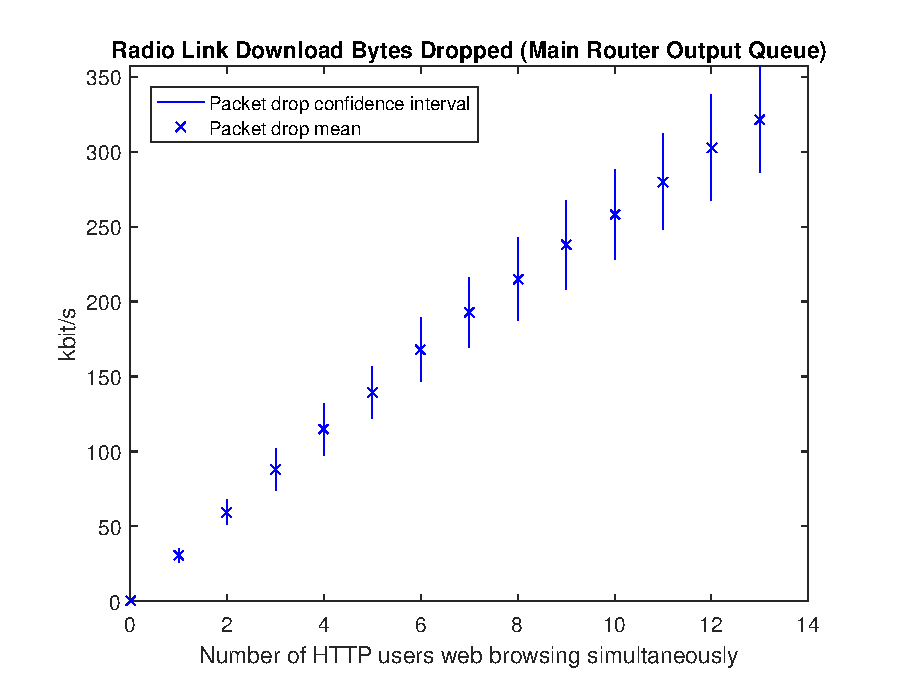
\includegraphics[width=0.9\textwidth]{on_main_router_drops.eps}
    \caption{kbits dropped per second at the main router output queue (see figure \ref{fig:network})}
    \label{fig:onMainRouterDrops}
    \end{center}
\end{figure}

On top of this, packets which are not dropped at the main router output queue often have a very long queuing time of up to 100 ms. While the mean queuing time ranges between 15 and 20 ms with six HTTP users, a high variance leads to a high number of unacceptable delays for the video connections. This means, simply increasing the maximum queuing length of the router is not an option. It may lead to less dropped packets but the video streams will still have a bad performance due to even higher delays caused by longer queues.

\chapter{Conclusion}
\label{chapter_conclusion}
By Nina Piontek and Daniel Plöger. \\

For both scenarios with the CCTV camera turned on and off, the FTP upload data rate turned out to be lower than expected. It was expected to be almost 10,000 kbit/s instead of a tenth of it. This behavior can not be explained with the simulation results and is assumed to be caused by faulty FTP protocol implementation in the simulation. This topic would need further investigation.

Even so it is not assumed that a higher FTP upload would have big impact on the other applications. Since it is the upstream direction it shares the link with the video conference upload and the CCTV camera, which both have negligible packet losses right now. With the FTP upload being close to the radio link data rate limit, there are still only three applications sharing this link direction, which is a number the router should be able to properly allocate.

As seen in the evaluation, the video stream down-link quality-of-service strongly depends on the number of HTTP users. Other applications do not seem to have high influence on the quality-of-service because without HTTP users and with all other applications active, both video streams work flawlessly. This means in conclusion that more bandwidth is needed in the down-link between main and remote router if more than six users should be able to browse on the web during a video conference with these parameters. It would also be possible to increase the quality of service of the video lecture by prioritizing the video data or by using a better video codec with lower data rates and higher tolerable delays. In summary, the radio link part of the network turns out to be the single bottleneck for the given scenario. 

	\bibliographystyle{plain}
	\bibliography{bibliography}
\end{document} 
